%******************************************************************************
% KOMA-Script article scrartcl
%******************************************************************************
\documentclass[12pt, b5paper]{article} 

% Add here all the packages that will be used in the document
%******************************************************************************
% Packages 
%******************************************************************************
% For hyperlinks 
\usepackage{url}

% Add no chapters to the article 
\usepackage[nochapters]{classicthesis}

% Setup the page geometry
\usepackage{geometry}
\geometry{a4paper, total={210mm, 297mm}, 
left=20mm, right=20mm, top=20mm, bottom=20mm}

% Use tikz to add watermarks to the document
\usepackage{blindtext,tikz}
\usetikzlibrary{calc}

% Use the classicthesis style for the style of the document
\usepackage[nochapters]{classicthesis} 

% Use the currvita style for the layout of the document
\usepackage[LabelsAligned]{currvita} 

% Required for adding links	and customizing them
\usepackage{hyperref} 

 % Set link colors
\hypersetup{colorlinks, breaklinks, urlcolor=Maroon, linkcolor=Maroon}


% Add a list of new commands 
%******************************************************************************
% Commands 
%******************************************************************************
\newcommand{\latex}{\LaTeX\xspace}
\newcommand{\tex}{\TeX\xspace}

\usepackage{listings}
\usepackage{color}
\usepackage{graphicx}
\usepackage{caption}
\usepackage{subcaption}

\graphicspath{{images/report5/}}

\definecolor{dkgreen}{rgb}{0,0.6,0}
\definecolor{gray}{rgb}{0.5,0.5,0.5}
\definecolor{mauve}{rgb}{0.58,0,0.82}

\lstset{frame=tb,
  language=Java,
  aboveskip=3mm,
  belowskip=3mm,
  showstringspaces=false,
  columns=flexible,
  basicstyle={\small\ttfamily},
  numbers=none,
  numberstyle=\tiny\color{gray},
  keywordstyle=\color{blue},
  commentstyle=\color{dkgreen},
  stringstyle=\color{mauve},
  breaklines=true,
  breakatwhitespace=true,
  tabsize=3
}

%******************************************************************************
% DOCUMENT STARTS HERE 
%******************************************************************************
\begin{document}

% TITLE 
\title{\rmfamily\normalfont\spacedallcaps{
Report \#{5}
}}

% PROJECT NAME -> ADD YOUR PROJECT NAME HERE
\author{{\small Automatic Mandible Segmentation Using VTK}}

% AUTOMATIC DATE -> DON'T CHANGE MANUALLY
\date{\footnotesize{\today}}

% MAKE THE TITLE -> DON'T CHANGE MANUALLY
\maketitle

% DON'T INCLUDE THE ABSTRACT FOR THE MOMENT
% % \begin{abstract}
% \noindent Abstract
% \end{abstract}
 
%******************************************************************************
% TABLE OF CONTENTS (uncomment to show / comment to hide)
%******************************************************************************     
% \tableofcontents


%******************************************************************************
% Report Content
%******************************************************************************
\section{Report Details}
\begin{center}
\begin{tabular}{ l | c }
\hline 
Report ID & 5   \\ % Change the sprint ID here 
\hline 
Report Duration & 1 Week \\ % Change the duration here 
\hline 
Beginning & 22.11.2016 \\ % Change the start data here
\hline 
End & 29.11.2016 \\ % Change the end data here
\hline 
\end{tabular}
\end{center}

%\section{Objectives}
\section{Original Objectives}
\begin{itemize}
\item Teeth Segmentation.
\item Visualization of Segmented Teeth.
\item GUI Implementation.
\item Saving Segmented Data in STL Format.
\end{itemize}

\section{Accomplished Objectives}
\subsection{Teeth Segmentation}
At first I used the labeling and connectivity algorithm that has been used in mandible segmentation to segment the teeth, and I changed some paramters which are the region of interest of the skull, and the threshold values. I did that for the segmented mandible and also for the skull before mandible segmentation and both of them works correctly. So no need to segment the mandible to be able to segment the teeth of mandible.

\subsection{Visualization of Segmented Teeth}
The segmented teeth using labeling and connectivity algorithm are shown in figure \ref{fig:CL}, It is clear that the data is badly visualized I don't know why, maybe due to thresholding that reduces the number of data points or there is another reason. So I have to used another way to get more clear and smooth teeth.

\vspace{1cm}
I found that extracting iso surfaces of the volume according to a specific iso value looks like thresholding process and then I need to have a connectivity filter to get the largest connected segment which is already exists in VTK library, It is \textit{vtkPolyDataConnectivityFilter} and I can set extraction mode to largest segment using \textit{SetExtractionModeToLargestRegion} method. This method gives me a very nice segmented teeth as shown in figure \ref{fig:PDCF}. I also found that I can use this method to segment the mandible too in few seconds. The extracted data is a poly data not image data so only surface rendering must be used for this method.

\begin{figure}
    \centering
    \begin{subfigure}[b]{0.45\textwidth}
        \centering
        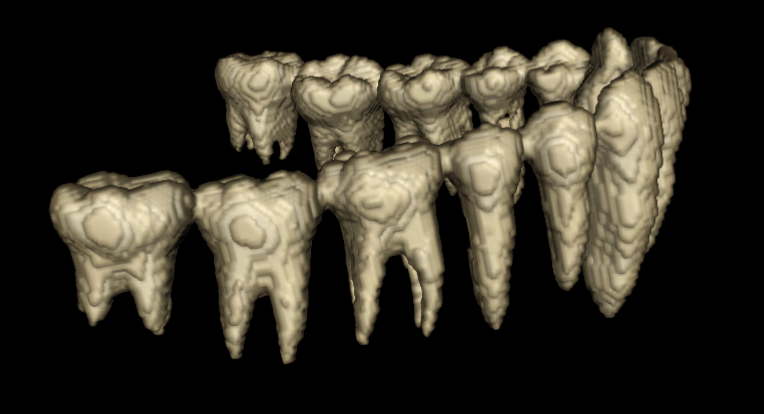
\includegraphics[width=\textwidth]{RCSO}
        \caption{Ray Casting}
    \end{subfigure}
    \hfill
    \begin{subfigure}[b]{0.45\textwidth}
        \centering
        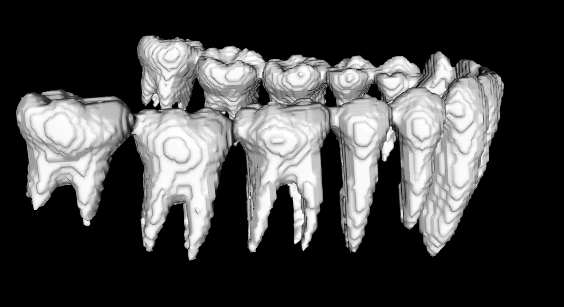
\includegraphics[width=\textwidth]{MCSO}
        \caption{Marching Cubes}
    \end{subfigure}
    \caption{Teeth Segmentation using labeling and connectivity algorithm.}
    \label{fig:CL}
\end{figure}


\begin{figure}
    \centering
    \begin{subfigure}[b]{0.5\textwidth}
        \centering
        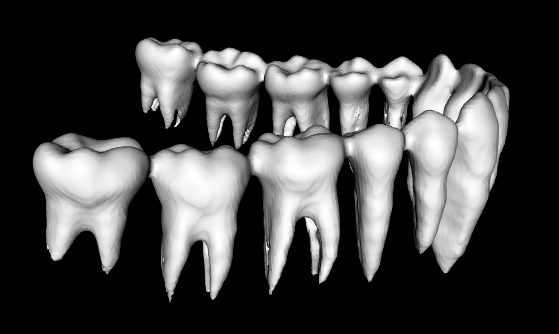
\includegraphics[width=\textwidth]{MCS2}
        \caption{First Side}
    \end{subfigure}
        \hfill
    \begin{subfigure}[b]{0.5\textwidth}
        \centering
        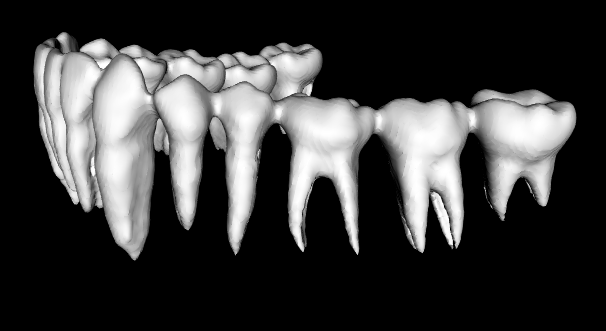
\includegraphics[width=\textwidth]{MCS1}
        \caption{Second Side}
    \end{subfigure}
    \hfill
    \begin{subfigure}[b]{0.5\textwidth}
        \centering
        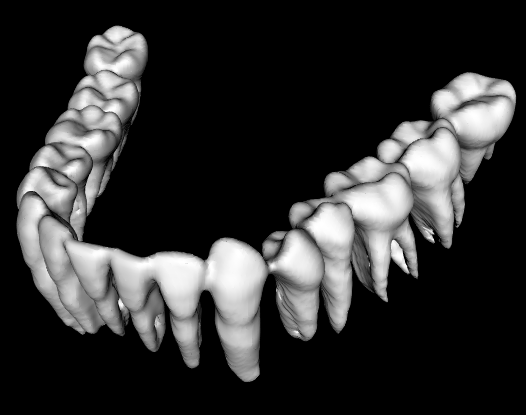
\includegraphics[width=\textwidth]{MCF1}
        \caption{Top View}
    \end{subfigure}
    \hfill
    \begin{subfigure}[b]{0.5\textwidth}
        \centering
        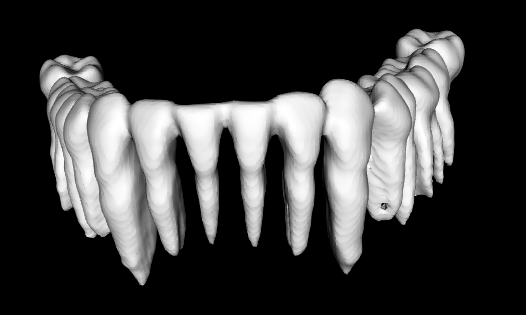
\includegraphics[width=\textwidth]{MCF2}
        \caption{Front View}
    \end{subfigure}
    \caption{Different Views of segmented Teeth with \textit{vtkPolyDataConnectivityFilter}}
    \label{fig:PDCF}
\end{figure}

\section{Missed Objectives}
\subsection{GUI Design}
Use Qt Gui libraries to make a simple graphical user interface that allow the user to load any volume and interactively set the segmentation parameters to segment desired object (mandible, or teeth).
\subsection{Saving Segmented Data in STL Format}
write the segmented data to STL file using \textit{vtkSTLWriter}. To be able to use it for processing without loading the whole dataset of the skull.

\section{Next Step}
\begin{itemize}
\item Do missed Objectives.
\item Optimization of the framework.
\end{itemize}
%******************************************************************************
% DOCUMENT ENDS HERE 
%******************************************************************************
\end{document}